\begin{table}
\begin{tabular}{l l l}
number of samples & mean & concentration\\ 
\hline
(true) & \includegraphics[width=0.6in]{output/1.models/samples_watson/watson_true.png} & 30.00\\ 
\hline
3 & \includegraphics[width=0.6in]{output/1.models/samples_watson/watson_est_3.png} & 19.37 \\ 
10 & \includegraphics[width=0.6in]{output/1.models/samples_watson/watson_est_10.png} & 37.72 \\ 
30 & 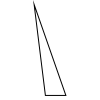
\includegraphics[width=0.6in]{output/1.models/samples_watson/watson_est_30.png} & 32.75 \\ 
100 & 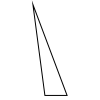
\includegraphics[width=0.6in]{output/1.models/samples_watson/watson_est_100.png} & 27.66 \\ 
300 & \includegraphics[width=0.6in]{output/1.models/samples_watson/watson_est_300.png} & 28.11 \\ 
1000 & \includegraphics[width=0.6in]{output/1.models/samples_watson/watson_est_1000.png} & 26.62 \\ 
\end{tabular}
\caption{Fitting the Watson distribution with different numbers of samples.}
\end{table}
